% Options for packages loaded elsewhere
\PassOptionsToPackage{unicode}{hyperref}
\PassOptionsToPackage{hyphens}{url}
%
\documentclass[
  english,
  man]{apa6}
\title{One- vs.~Two-Step Approach in Regularized Bayesian Structural Equation Modeling (SEM)}
\author{\phantom{0}}
\date{}

\usepackage{amsmath,amssymb}
\usepackage{lmodern}
\usepackage{iftex}
\ifPDFTeX
  \usepackage[T1]{fontenc}
  \usepackage[utf8]{inputenc}
  \usepackage{textcomp} % provide euro and other symbols
\else % if luatex or xetex
  \usepackage{unicode-math}
  \defaultfontfeatures{Scale=MatchLowercase}
  \defaultfontfeatures[\rmfamily]{Ligatures=TeX,Scale=1}
\fi
% Use upquote if available, for straight quotes in verbatim environments
\IfFileExists{upquote.sty}{\usepackage{upquote}}{}
\IfFileExists{microtype.sty}{% use microtype if available
  \usepackage[]{microtype}
  \UseMicrotypeSet[protrusion]{basicmath} % disable protrusion for tt fonts
}{}
\makeatletter
\@ifundefined{KOMAClassName}{% if non-KOMA class
  \IfFileExists{parskip.sty}{%
    \usepackage{parskip}
  }{% else
    \setlength{\parindent}{0pt}
    \setlength{\parskip}{6pt plus 2pt minus 1pt}}
}{% if KOMA class
  \KOMAoptions{parskip=half}}
\makeatother
\usepackage{xcolor}
\IfFileExists{xurl.sty}{\usepackage{xurl}}{} % add URL line breaks if available
\IfFileExists{bookmark.sty}{\usepackage{bookmark}}{\usepackage{hyperref}}
\hypersetup{
  pdftitle={One- vs.~Two-Step Approach in Regularized Bayesian Structural Equation Modeling (SEM)},
  pdflang={en-EN},
  hidelinks,
  pdfcreator={LaTeX via pandoc}}
\urlstyle{same} % disable monospaced font for URLs
\usepackage{graphicx}
\makeatletter
\def\maxwidth{\ifdim\Gin@nat@width>\linewidth\linewidth\else\Gin@nat@width\fi}
\def\maxheight{\ifdim\Gin@nat@height>\textheight\textheight\else\Gin@nat@height\fi}
\makeatother
% Scale images if necessary, so that they will not overflow the page
% margins by default, and it is still possible to overwrite the defaults
% using explicit options in \includegraphics[width, height, ...]{}
\setkeys{Gin}{width=\maxwidth,height=\maxheight,keepaspectratio}
% Set default figure placement to htbp
\makeatletter
\def\fps@figure{htbp}
\makeatother
\setlength{\emergencystretch}{3em} % prevent overfull lines
\providecommand{\tightlist}{%
  \setlength{\itemsep}{0pt}\setlength{\parskip}{0pt}}
\setcounter{secnumdepth}{-\maxdimen} % remove section numbering
% Make \paragraph and \subparagraph free-standing
\ifx\paragraph\undefined\else
  \let\oldparagraph\paragraph
  \renewcommand{\paragraph}[1]{\oldparagraph{#1}\mbox{}}
\fi
\ifx\subparagraph\undefined\else
  \let\oldsubparagraph\subparagraph
  \renewcommand{\subparagraph}[1]{\oldsubparagraph{#1}\mbox{}}
\fi
\newlength{\cslhangindent}
\setlength{\cslhangindent}{1.5em}
\newlength{\csllabelwidth}
\setlength{\csllabelwidth}{3em}
\newlength{\cslentryspacingunit} % times entry-spacing
\setlength{\cslentryspacingunit}{\parskip}
\newenvironment{CSLReferences}[2] % #1 hanging-ident, #2 entry spacing
 {% don't indent paragraphs
  \setlength{\parindent}{0pt}
  % turn on hanging indent if param 1 is 1
  \ifodd #1
  \let\oldpar\par
  \def\par{\hangindent=\cslhangindent\oldpar}
  \fi
  % set entry spacing
  \setlength{\parskip}{#2\cslentryspacingunit}
 }%
 {}
\usepackage{calc}
\newcommand{\CSLBlock}[1]{#1\hfill\break}
\newcommand{\CSLLeftMargin}[1]{\parbox[t]{\csllabelwidth}{#1}}
\newcommand{\CSLRightInline}[1]{\parbox[t]{\linewidth - \csllabelwidth}{#1}\break}
\newcommand{\CSLIndent}[1]{\hspace{\cslhangindent}#1}
% This preamble allows to remove the redundant title page from papaja's output.pdf
\usepackage{atbegshi}% http://ctan.org/pkg/atbegshi
\AtBeginDocument{\AtBeginShipoutNext{\AtBeginShipoutDiscard}}
% Manuscript styling
\usepackage{upgreek}
\captionsetup{font=singlespacing,justification=justified}

% Table formatting
\usepackage{longtable}
\usepackage{lscape}
% \usepackage[counterclockwise]{rotating}   % Landscape page setup for large tables
\usepackage{multirow}		% Table styling
\usepackage{tabularx}		% Control Column width
\usepackage[flushleft]{threeparttable}	% Allows for three part tables with a specified notes section
\usepackage{threeparttablex}            % Lets threeparttable work with longtable

% Create new environments so endfloat can handle them
% \newenvironment{ltable}
%   {\begin{landscape}\centering\begin{threeparttable}}
%   {\end{threeparttable}\end{landscape}}
\newenvironment{lltable}{\begin{landscape}\centering\begin{ThreePartTable}}{\end{ThreePartTable}\end{landscape}}

% Enables adjusting longtable caption width to table width
% Solution found at http://golatex.de/longtable-mit-caption-so-breit-wie-die-tabelle-t15767.html
\makeatletter
\newcommand\LastLTentrywidth{1em}
\newlength\longtablewidth
\setlength{\longtablewidth}{1in}
\newcommand{\getlongtablewidth}{\begingroup \ifcsname LT@\roman{LT@tables}\endcsname \global\longtablewidth=0pt \renewcommand{\LT@entry}[2]{\global\advance\longtablewidth by ##2\relax\gdef\LastLTentrywidth{##2}}\@nameuse{LT@\roman{LT@tables}} \fi \endgroup}

% \setlength{\parindent}{0.5in}
% \setlength{\parskip}{0pt plus 0pt minus 0pt}

% \usepackage{etoolbox}
\makeatletter
\patchcmd{\HyOrg@maketitle}
  {\section{\normalfont\normalsize\abstractname}}
  {\section*{\normalfont\normalsize\abstractname}}
  {}{\typeout{Failed to patch abstract.}}
\patchcmd{\HyOrg@maketitle}
  {\section{\protect\normalfont{\@title}}}
  {\section*{\protect\normalfont{\@title}}}
  {}{\typeout{Failed to patch title.}}
\makeatother
\shorttitle{One- vs. Two-Step Approach in Regularized Bayesian SEM}
\keywords{\newline\indent Word count: X}
\DeclareDelayedFloatFlavor{ThreePartTable}{table}
\DeclareDelayedFloatFlavor{lltable}{table}
\DeclareDelayedFloatFlavor*{longtable}{table}
\makeatletter
\renewcommand{\efloat@iwrite}[1]{\immediate\expandafter\protected@write\csname efloat@post#1\endcsname{}}
\makeatother
\usepackage{csquotes}
\ifXeTeX
  % Load polyglossia as late as possible: uses bidi with RTL langages (e.g. Hebrew, Arabic)
  \usepackage{polyglossia}
  \setmainlanguage[]{english}
\else
  \usepackage[main=english]{babel}
% get rid of language-specific shorthands (see #6817):
\let\LanguageShortHands\languageshorthands
\def\languageshorthands#1{}
\fi
\ifLuaTeX
  \usepackage{selnolig}  % disable illegal ligatures
\fi


\affiliation{\phantom{0}}

\begin{document}
\maketitle


% move text to bottom of page
\vfill
Research Proposal \\
Michael Koch (6412157)\\
Methodology and Statistics for the Behavioral, Biomedical, and Social Sciences \\
Supervisor: Dr. Sara van Erp \\ 
Email: j.m.b.koch@students.uu.nl \\
Word Count: 750 \\
Intented Journal of Publication: Structural Equation Modeling

% make page numbers start from second page 
\pagenumbering{arabic}
\setcounter{page}{0}
\thispagestyle{empty}
% make page numbers from second page 
\pagestyle{plain}

\clearpage

In the context of \emph{Confirmatory Factor Analysis (CFA)} a popular model falling under the broader class of \emph{Structural Equation Modeling (SEM)}, the desire for model simplicity manifest itself in the common practice of fitting models with a simple structure. Here, so-called ``cross-loadings,'' , are fixed to zero, which serves the purpose of both identifying the model, and yielding an end-result that can be interpreted straightforwardly. However, often times, this practice leads to poor model fit. Consequently, researchers commonly free some cross-loadings based on modification indices to improve model fit, a practice that is flawed for a variety of reason, among which risking capitalization on chance {[}REFs, there's plenty{]}.

As solution, Muthen and Asparouhov (2012) proposed \emph{Bayesian SEM}. For CFA models, they argued that rather than fixing all cross-loadings to zero, one should make a more realistic and flexible assumption.
Formally, this is achieved by setting the so called Small Variance Prior for the cross-loadings, which is a normal distribution with mean zero and a very small variance \(\sigma\) (e.g.: \(\sigma = 0.01, \  \sigma = 0.001\))

\[\mathcal{N}(0, \sigma)\]

By tuning the variance of the prior, one is able to fit a systematically, continuously varying sequence of models. This, in turn, allows for a more continuous process of model identification and model selection.

However, a core issue with the approach by Muthen and Asparouhov (2012) is that applying the Small Variance Prior requires a 2-step approach (Lu, Chow, \& Loken, 2016). Not only the cross-loadings close to zero, that can be considered irrelevant, are shrunken to zero, as desired. Also the cross-loadings that are further from zero, and are therefore likely to play a more crucial role in accurately modeling the factor structure of the data are shrunken substantially, which introduces bias. Therefore, more advanced priors need to be identified that can outperform the small-variance prior \emph{in a single step}.

A promising candidate

\emph{Horseshoe prior} (Carvalho, Polson, \& Scott, 2010):
Practically no shrinkage for large coefficients, shrinkage to zero for small coefficients
\emph{Global} component \(\lambda\), shrinking all parameters towards zero, \emph{local} component \(\tau_j\) allowing large parameters to escape shrinkage

\begin{equation} 
  \beta_j | \tau^2_j, \sim \mathcal{N}(0, \tau^2_j )  
  
  \tau_j \sim C^+(0, \lambda) \ for \ j = 1, \ ..., \ p  
  
  \lambda| \sigma \sim C^+(0, \sigma) 
\end{equation}

The \emph{Regularized Horseshoe} prior builds on the horseshoe prior, by, which is achieve by \ldots{} (See Equation 4).

\[\beta_j | \hat{\tau}, \lambda \sim \mathcal{N}(0, \hat{\tau}^2 \lambda), \ with \ \hat{\tau}^2 = \frac{c^2t_j^2}{c^2 + \lambda^2 \tau_j^2} \]
\[\lambda | \lambda_0^2 \sim \mathcal{N}(0, \lambda_0^2), \ with \  \lambda_0 = \frac{p_0}{p-p_0}\frac{\sigma}{\sqrt{N}}\]
\[\tau_j \sim \mathcal{C^+}(0, 1)\]
\[c^2 | \nu, s^2 \sim \mathcal{IG}(\nu/2, \  \nu s^2/2)\]

In sum, the Regularized Horseshoe prior is characterized by a unique combination of desired traits. This raises the expectation that it would outperform the Small Variance Prior in selecting the correct loading structure of a CFA model, within a single step. However, while previous research has shown promising results with the Regularized Horseshoe Prior in the selection of the correct predictor structure of Regression models {[}REFs?!{]}, no previous research has validated its performance in the selection of the factor structure in CFA.

To fill this gap, the aim of this study is to compare the Regularized Horseshoe Prior to the Small Variance Prior in their performance in selecting the true factor structure in Confirmatory Factor Analysis (CFA).

\begin{figure}
\centering
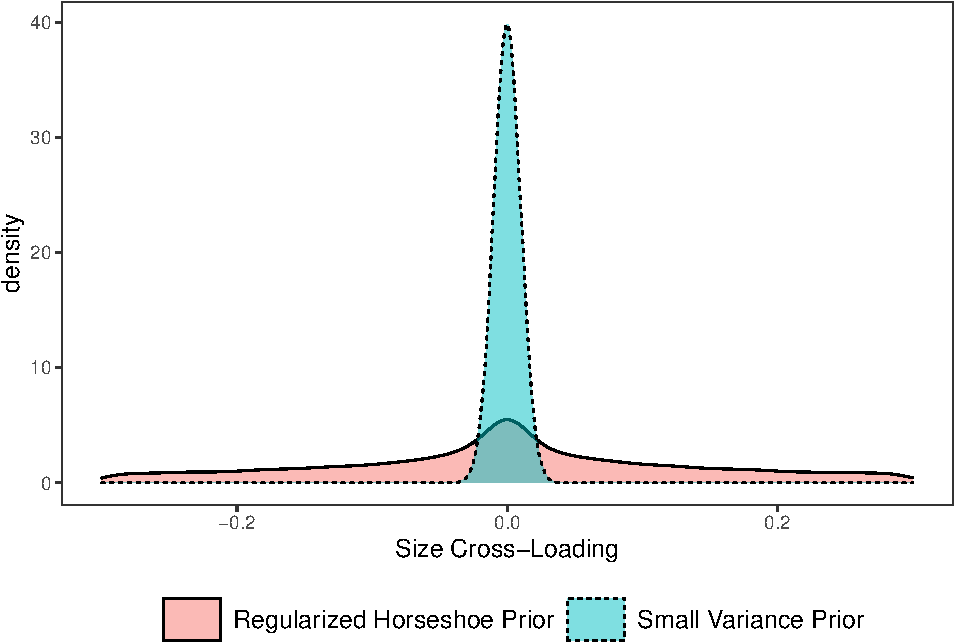
\includegraphics{JMBKoch_Proposal_files/figure-latex/unnamed-chunk-1-1.pdf}
\caption{\label{fig:unnamed-chunk-1}Density Plots of the Regularization Priors of Interest}
\end{figure}

\hypertarget{analytic-strategy}{%
\subsection{Analytic Strategy}\label{analytic-strategy}}

A Monte Carlo simulation study is conducted using stan (Carpenter et al., 2017).
True Positives vs.~False Positives in estimating truly non-zero cross-loadings as non-zero are considered as main outcome (ROC).
Conditions are based on (Lu et al., 2016) and will include two factor structures (1 non-zero cross-loading, several non-zero cross-loadings), three sample sizes (100, 200, 300), and three magnitudes of the cross-loadings (0.1, 0.2, 0.3). These sizes are \ldots{}

\clearpage

\hypertarget{references}{%
\section{References}\label{references}}

\begingroup
\setlength{\parindent}{-0.5in}
\setlength{\leftskip}{0.5in}

\hypertarget{refs}{}
\begin{CSLReferences}{1}{0}
\leavevmode\vadjust pre{\hypertarget{ref-carpenter_stan_2017}{}}%
Carpenter, B., Gelman, A., Hoffman, M. D., Lee, D., Goodrich, B., Betancourt, M., \ldots{} Riddell, A. (2017). Stan: {A} {Probabilistic} {Programming} {Language}. \emph{Journal of Statistical Software}, \emph{76}(1), 1--32. \url{https://doi.org/10.18637/jss.v076.i01}

\leavevmode\vadjust pre{\hypertarget{ref-carvalho_horseshoe_2010}{}}%
Carvalho, C. M., Polson, N. G., \& Scott, J. G. (2010). The horseshoe estimator for sparse signals. \emph{Biometrika}, \emph{97}(2), 465--480. \url{https://doi.org/10.1093/biomet/asq017}

\leavevmode\vadjust pre{\hypertarget{ref-lu_bayesian_2016}{}}%
Lu, Z.-H., Chow, S.-M., \& Loken, E. (2016). Bayesian {Factor} {Analysis} as a {Variable}-{Selection} {Problem}: {Alternative} {Priors} and {Consequences}. \emph{Multivariate Behavioral Research}, \emph{51}(4), 519--539. \url{https://doi.org/10.1080/00273171.2016.1168279}

\leavevmode\vadjust pre{\hypertarget{ref-muthen_bayesian_2012}{}}%
Muthen, B., \& Asparouhov, T. (2012). Bayesian {SEM}: {A} more flexible representation of substantive theory, 78. \url{https://doi.org/10.1037/a0026802}

\end{CSLReferences}

\endgroup


\end{document}
